%!TEX root = main.tex
\paragraph{Boundary integral formulation of electrostatics in molecular solvation}\label{s:formulation}

Biomolecules in an ionic solvent or water can be represented with a model where the solvent is a continuous dielectric: the so-called implicit-solvent model.
The molecule (solute) is a dielectric cavity with partial charges at the atomic locations,  represented as a collection of Dirac delta functions.
In  the sketch of Figure \ref{fig:implicit_solvent}, the molecular cavity is region $\Omega_1$, the infinite medium  is $\Omega_2$, and the point charges are $q_k$.
The interface $\Gamma$ represents the molecular surface and can be determined through several approaches: van der Waals radii, Gaussian surface, solvent-accessible surface, and solvent-excluded surface. 
We use the latter.
A solvent-excluded surface is built by tracking the contact points of a (virtual) spherical probe of  $\sim$ 1.4 \AA\ in radius, the size of a water molecule, as it rolls around the solute's atoms (with their corresponding van der Waals radii). 
In this setup, we can compute the change in electrostatic potential as the interior region is charged up with the solute's partial charges.
The solvent usually consists of water (dielectric constant $\epsilon_2\approx80$) with salt ions that are free to move around, forced by the electric field. 
At equilibrium, the salt ions are in a Boltzmann distribution, leading to the linearized Poisson-Boltzmann equation for the potential in $\Omega_2$, considering a screening factor known as the Debye length ($\kappa$.) 
The electrostatic potential in the solute cavity follows Poisson's equation in a low dielectric medium ($\epsilon_1\approx2\textrm{--}4$), with the solute's point charges as sources.
With interface conditions on the molecular surface $\Gamma$, where the potential and electric displacement must be continuous, this results in the following system of equations:
%
\begin{align} \label{eq:pde}
\nabla^2\phi_1 &= \frac{1}{\epsilon_1}\sum_k q_k\delta(\mathbf{r},\mathbf{r}_k) \text{ in the solute ($\Omega_1$),}\nonumber\\
(\nabla^2-\kappa^2)\phi_2 &= 0 \text{ in the solvent ($\Omega_2$),}\nonumber\\
\phi_1 &= \phi_2 \quad \epsilon_1\frac{\partial \phi_1}{\partial\mathbf{n}} = \epsilon_2\frac{\partial \phi_2}{\partial\mathbf{n}} \text{ on the interface ($\Gamma$)}.
\end{align}
%

%
\begin{figure}
\centering
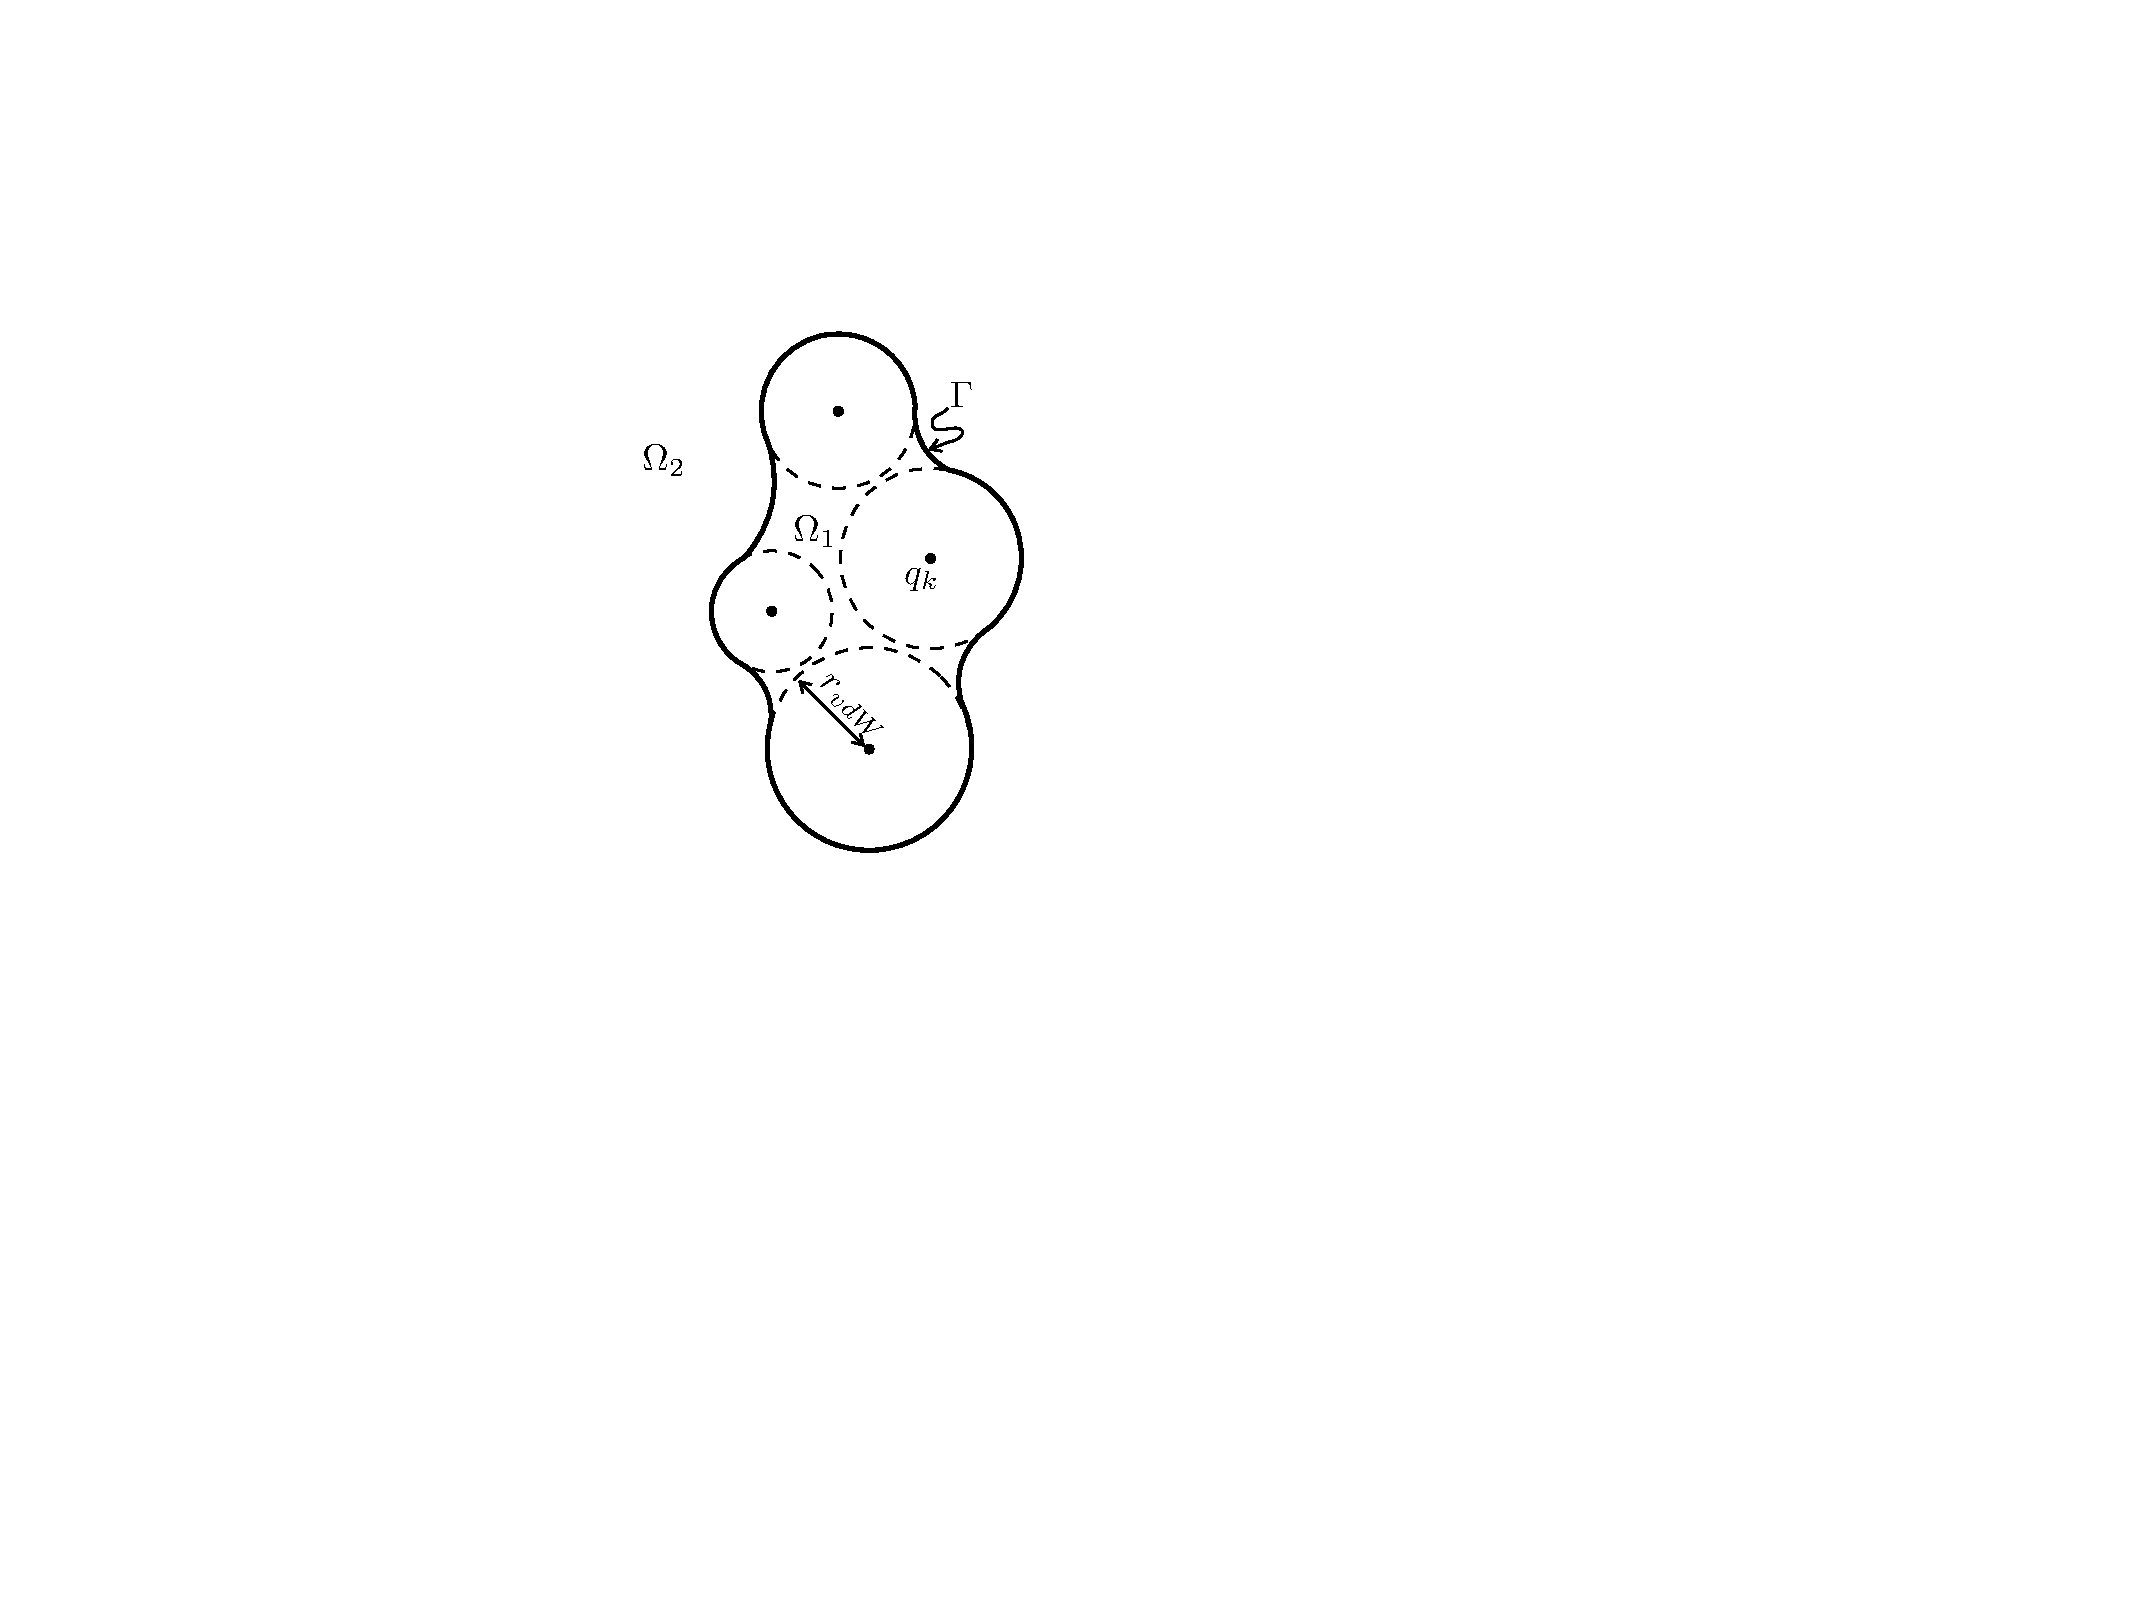
\includegraphics[width=0.25\textwidth]{implicit_solvent.pdf}
\caption{Representation of a dissolved molecule with the implicit-solvent model. The solute ($\Omega_1$) and solvent ($\Omega_2$) regions are interfaced by the solvent-excluded surface ($\Gamma$), and $q_k$ and $r_{vdW}$ are the atomic charge and radii, respectively.}
\label{fig:implicit_solvent}
\end{figure}

Equation \eqref{eq:pde} can be re-written as an integral equation on $\Gamma$ via Green's second identity, yielding:
%
\begin{align} \label{eq:volume_potential}
\phi_{1}+ K_{L}^{\Omega_1}(\phi_{1,\Gamma}) -  V_{L}^{\Omega_1} \left(\frac{\partial}{\partial \mathbf{n}}  \phi_{1,\Gamma}  \right) & = \frac{1}{\epsilon_1} \sum_{k=0}^{N_q}  \frac{q_k}{4\pi|\mathbf{r}_{\Omega_1} - \mathbf{r}_k|}  \quad \text{on $\Omega_1$,} \nonumber \\
\phi_{2} - K_{Y}^{\Omega_2}(\phi_{2,\Gamma}) + V_{Y}^{\Omega_2} \left( \frac{\partial}{\partial \mathbf{n}} \phi_{2,\Gamma} \right) & = 0 \quad \text{on $\Omega_2$,}
\end{align}
%
where $\phi_{1,\Gamma} = \phi_1(\mathbf{r}_\Gamma)$ and $\phi_{2,\Gamma} = \phi_2(\mathbf{r}_\Gamma)$ are evaluated on $\Gamma$ approaching from $\Omega_1$ and $\Omega_2$, respectively. $K$ and $V$ are the double- and single-layer potentials for the Laplace (subscript $L$) and modified Helmholtz (Yukawa, subscript $Y$) kernels, defined as:
%
\begin{align}\label{eq:single_double}
V^\Omega_{L,Y}(\varphi) = \oint_\Gamma g_{L,Y}(\mathbf{r}_\Omega,\mathbf{r}')\varphi(\mathbf{r}')d\mathbf{r}'\nonumber\\
K^\Omega_{L,Y}(\varphi) = \oint_\Gamma \frac{\partial g_{L,Y}}{\partial\mathbf{n}'}(\mathbf{r}_\Omega,\mathbf{r}')\varphi(\mathbf{r}')d\mathbf{r}',\nonumber\\
\end{align}
%
where $\varphi(\mathbf{r})$ is a distribution over $\Gamma$, and $g_L(\mathbf{r},\mathbf{r}')=\frac{1}{4\pi|\mathbf{r}-\mathbf{r}'|}$ and $g_Y(\mathbf{r},\mathbf{r}')=\frac{e^{-\kappa|\mathbf{r}-\mathbf{r}'|}}{4\pi|\mathbf{r}-\mathbf{r}'|}$ are the free-space Green's function of the Laplace and linearized Poisson-Boltzmann equations, respectively. 

We can use Equation \eqref{eq:volume_potential} to compute $\phi_\Gamma$ and $\partial\phi_\Gamma/\partial\mathbf{n}$ with either the \emph{direct}~\cite{YoonLenhoff1990} or \emph{derivative}~\cite{JufferETal1991} (also known as \emph{Juffer}) formulations.
The simpler direct formulation results from evaluating $\phi_1$ and $\phi_2$ in the limit as $\mathbf{r}$ approaches $\Gamma$, and applying the interface conditions from Equation \eqref{eq:pde}, giving:
%
\begin{align} \label{eq:direct}
\frac{\phi_{1,\Gamma}}{2}+ K_{L}^{\Gamma}(\phi_{1,\Gamma}) -  V_{L}^{\Gamma} \left(\frac{\partial}{\partial \mathbf{n}}  \phi_{1,\Gamma}  \right) & = \frac{1}{\epsilon_1} \sum_{k=0}^{N_q}  \frac{q_k}{4\pi|\mathbf{r}_{\Gamma} - \mathbf{r}_k|} \nonumber \\
\frac{\phi_{1,\Gamma}}{2} - K_{Y}^{\Gamma}(\phi_{1,\Gamma}) + \frac{\epsilon_1}{\epsilon_2}V_{Y}^{\Gamma} \left( \frac{\partial}{\partial \mathbf{n}} \phi_{1,\Gamma} \right) & = 0
\end{align}
%
This formulation is ill-conditioned, since the condition number of the resulting matrix grows unbounded with the number of discretization elements. 
An alternative with better conditioning was derived by Juffer \emph{et al.} \cite{JufferETal1991} by taking the normal derivative of Equation \eqref{eq:volume_potential}, and coupling both $\phi$ and $\partial\phi/\partial\mathbf{n}$ on the boundary as follows:

\begin{align}\label{eq:juffer}
\frac{\phi_{1,\Gamma}}{2}\left(1+\frac{\epsilon_2}{\epsilon_1}\right) - \left(\frac{\epsilon_2}{\epsilon_1}K_Y^\Gamma - K_L^\Gamma\right)(\phi_{1,\Gamma}) &+ \left(V_Y^\Gamma - V_L^\Gamma\right)\left( \frac{\partial}{\partial \mathbf{n}} \phi_{1,\Gamma} \right)\nonumber\\ 
&= \sum_{k=0}^{N_q}  \frac{q_k}{4\pi\epsilon_1|\mathbf{r}_{\Gamma} - \mathbf{r}_k|} \nonumber \\
- \left(W_Y^\Gamma - W_L^\Gamma\right)(\phi_{1,\Gamma}) +  \frac{1}{2}\frac{\phi_{1,\Gamma}}{\partial\mathbf{n}}\left(1+\frac{\epsilon_1}{\epsilon_2}\right) &+ \left(\frac{\epsilon_1}{\epsilon_2}K_Y^{\prime\Gamma} - K_L^{\prime\Gamma}\right)\left( \frac{\partial}{\partial \mathbf{n}} \phi_{1,\Gamma} \right)\nonumber\\ 
&= \sum_{k=0}^{N_q}  \frac{\partial}{\partial\mathbf{n}_\mathbf{r}}\left(\frac{q_k}{4\pi\epsilon_1|\mathbf{r}_{\Gamma} - \mathbf{r}_k|}\right) \nonumber \\
\end{align}
%
Here, we use the adjoint double-layer ($K'$) and hypersingular ($W$) operators, which are defined as
%
\begin{align}\label{eq:adj_hyp}
K^{\prime\Gamma}_{L,Y}(\varphi) = \oint_\Gamma \frac{g_{L,Y}}{\partial\mathbf{n}}(\mathbf{r}_\Gamma,\mathbf{r}')\varphi(\mathbf{r}')d\mathbf{r}'\nonumber\\
W^\Gamma_{L,Y}(\varphi) = \oint_\Gamma \frac{\partial^2 g_{L,Y}}{\partial\mathbf{n}'\partial\mathbf{n}}(\mathbf{r}_\Gamma,\mathbf{r}')\varphi(\mathbf{r}')d\mathbf{r}'\nonumber\\
\end{align}
%
A slightly modified version of Equation \eqref{eq:juffer} is used in the work from Lu and coworkers~\cite{LuETal2006,LuETal2009,ZhangETal2019}, where they scale the expressions by $\epsilon_1/\epsilon_2$, and solve for the exterior field. This gives
%
\begin{align}\label{eq:lu}
\frac{\phi_{2,\Gamma}}{2}\left(\frac{\epsilon_1}{\epsilon_2}+1\right) - \left(K_Y^\Gamma - \frac{\epsilon_1}{\epsilon_2}K_L^\Gamma\right)(\phi_{2,\Gamma}) &+ \left(V_Y^\Gamma - V_L^\Gamma\right)\left( \frac{\partial}{\partial \mathbf{n}} \phi_{2,\Gamma} \right)\nonumber\\ 
&= \sum_{k=0}^{N_q}  \frac{q_k}{4\pi\epsilon_2|\mathbf{r}_{\Gamma} - \mathbf{r}_k|} \nonumber \\
- \frac{\epsilon_1}{\epsilon_2}\left(W_Y^\Gamma - W_L^\Gamma\right)(\phi_{2,\Gamma}) +  \frac{1}{2}\frac{\phi_{2,\Gamma}}{\partial\mathbf{n}}\left(1+\frac{\epsilon_1}{\epsilon_2}\right) &+ \left(\frac{\epsilon_1}{\epsilon_2}K_Y^{\prime\Gamma} - K_L^{\prime\Gamma}\right)\left( \frac{\partial}{\partial \mathbf{n}} \phi_{2,\Gamma} \right)\nonumber\\ 
&= \sum_{k=0}^{N_q}  \frac{\partial}{\partial\mathbf{n}_\mathbf{r}}\left(\frac{q_k}{4\pi\epsilon_2|\mathbf{r}_{\Gamma} - \mathbf{r}_k|}\right) \nonumber \\
\end{align}

As we charge up the cavity, the solvent ions rearrange and polarize.
The resulting electrostatic potential is called a \emph{reaction} potential ($\phi_{reac}$), and we can write the following decomposition in $\Omega_1$ :
%
\begin{equation}
\phi_1 = \phi_{reac} + \phi_{coul},
\end{equation}
%
where $\phi_{coul}$ is the Coulombic potential from the solute point charges only.
Having $\phi_{1,\Gamma}$ and $\partial\phi_{1,\Gamma}/\partial\mathbf{n}$ from Equation \eqref{eq:direct} or Equation \eqref{eq:juffer}, we can compute $\phi_{reac}$ by subtracting out the Coulombic contribution in the right-hand side of Equation \eqref{eq:volume_potential}:
%
\begin{equation}\label{eq:phi_reac}
\phi_{reac} = -K_{L}^{\Omega_1}(\phi_{1,\Gamma}) +  V_{L}^{\Omega_1} \left(\frac{\partial}{\partial \mathbf{n}}  \phi_{1,\Gamma}  \right) 
\end{equation}

The thermodynamic work required to dissolve a molecule, known as solvation free energy, is usually divided into nonpolar and polar components.
The nonpolar part generates the empty solute-shaped cavity in the solvent, which is then charged by placing the partial charges inside the cavity, giving rise to a polar term in the energy. 
The work in charging is performed under $\phi_{reac}$, and it can be computed as:
%
\begin{equation} \label{eq:energy}
\Delta G^{polar}_{solv} = \frac{1}{2}\int_{\Omega_1} \rho\phi_{reac}d\mathbf{r} = \frac{1}{2}\sum_{k=1}^{N_q}q_k\phi_{reac}(\mathbf{r}_k).
\end{equation}
